%%%%%%
%
% $Autor: Wings $
% $Datum: 2020-01-18 11:15:45Z $
% $Pfad: WuSt/Skript/Produktspezifikation/powerpoint/ImageProcessing.tex $
% $Version: 4620 $
%
%%%%%%

%Quelle: https://towardsdatascience.com/deep-learning-framework-power-scores-2018-23607ddf297a
%\url{https://www.kdnuggets.com/2019/05/which-deep-learning-framework-growing-fastest.html}
% \url{https://www.kdnuggets.com/2017/08/pytorch-tensorflow.html}

%todo    \href{https://docs.aws.amazon.com/de_de/machine-learning/latest/dg/step-1-download-edit-and-upload-data.html}{Amazon ML}
%todo https://www.ibm.com/de-de/products/trials


\chapter{Frameworks and Libraries}
\index{Frameworks}
\index{Bibiotheken}


%todo
%todo \section{Kriterien}
%todo https://towardsdatascience.com/deep-learning-framework-power-scores-2018-23607ddf297a


As a programming language for data science, Python represents a compromise between the R language, which focuses on data analysis and visualisation, and Java, which forms the backbone of many large-scale applications. This flexibility means that Python can act as a single tool that brings your entire workflow together.

Python is often the first choice for developers who need to apply statistical techniques or data analysis to their work, or for data scientists whose tasks need to be integrated into web applications or production environments. Python particularly shines in the area of machine learning. The combination of machine learning libraries and flexibility makes Python unique. Python is best suited for developing sophisticated models and predictive modules that can be directly integrated into production systems.

One of Python's greatest strengths is its extensive library. Libraries are sets of routines and functions written in a specific language. A robust set of libraries can make the job of developers immensely easier to perform complex tasks without having to rewrite many lines of code. 



\section{Development Environment}


\subsection{Jupyter-Notebook}
\index{Jupyter-Notebook}

Mhe Jupyter Notebook application can be used to create a file in a web browser. The advantage here is that programmes can be divided into smaller programme sections and executed section by section. This makes working very interactive. The notebook also offers the possibility of annotating Python programme codes with additional text.
annotations. \cite{Buxmann:2019}




\section{Frameworks}







\subsection{TensorFlow}
\index{TensorFlow}


The TensorFlow framework, which is supported by Google, is the undisputed top dog. It has the most GitHub activity, Google searches, Medium articles, books on Amazon and ArXiv articles. It also has the most developers using it, and is listed in the most online job descriptions. \cite{GoogleTensorFlow:2019}

Variant also exist for TensorFlow that is specific to a hardware. For example, NVIDIA graphics cards are addressed by a variant with \ac{cuda} and Intel also has an optimised variant. However, you may have to do without the latest version.

TensorFlow Lite, the small device version, brings model execution to a variety of devices, including mobile devices and IoT, and provides more than a 3x increase in inference speed compared to the original TensorFlow. 

TensorFlow uses data flow graphs to represent computation, shared state, and the operations that mutate that state. By fully representing the dependencies of each step of the computation, parts of the computation can be reliably parallelised \cite{Abadi:2016}. 
Originally, TensorFlow was to be used for Google's internal use, but was
released in November 2015 under the Apache 2.0 open source licence.
Since then, TensorFlow has brought together a variety of tools, libraries and communities.
TensorFlow provides low-level interfaces for programming languages such as Python, Java,
C++ and Go. The mid-level and high-level APIs provide functions for creating, training, saving and loading models,
training, saving and loading models. \cite{Chollet:2018} %[Men16] 

\begin{figure}[htb]
	\centering
	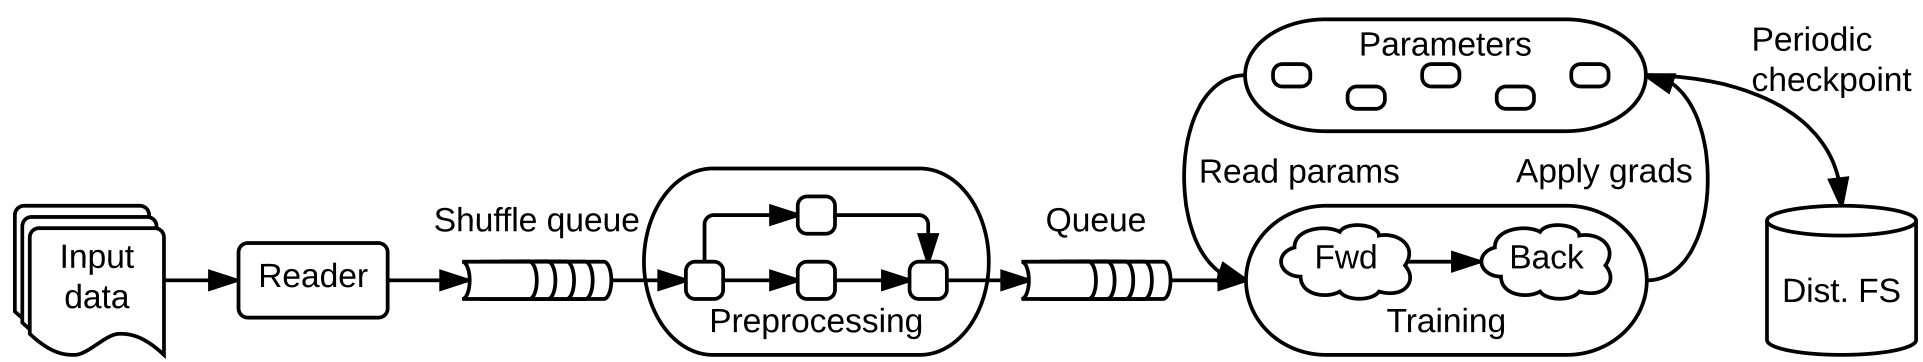
\includegraphics[width=\textwidth]{CUDA/tensorflow-flow-graph.PNG}
	\caption[Tensorflow Datenflussdiagramm]{Tensorflow Datenflussdiagramm \cite{Abadi:2016}}
	\label{fig:tensorflow-flow}
\end{figure}



\subsection{TensorFlow Lite}
\index{TensorFlow Lite}

Tensorflow Lite is an optimised environment for TensorFlow models for mobile devices and the \ac{iot}. Essentially, it consists of two components: the converter, which converts pre-trained TensorFlow models into optimised TensorFlow Lite models, and the interpreter, which enables optimised execution on the various end devices. The goal here is to reduce the size of the existing models and to reduce latency on less powerful devices \cite{GoogleTensorFlowLiteGuide:2020}.

\subsection{TensorRT}\label{sec:tensorrt}
\index{TensorRT}

TensorRT is a neural network runtime environment based on \ac{cuda}, which specialises in optimising the performance of neural networks \cite{TensorRT:2015}. This is achieved by reducing the computational accuracy from \ac{fp32} to \ac{fp16} resp. \ac{int8}. Since the remaining interference accuracy is sufficient for most use cases, the speed can be significantly increased with this method \cite{Gysel:2016}. When optimising the network, the operators used are replaced by TensorRT operators, which can only be executed within a TensorRT environment.


\subsection{Keras}
\index{Keras}

Keras is a high-level \ac{api} application programming interface (API) for neural networks built in Python and running on TensorFlow, Theano or CNTK. It enables the definition and training of different deep learning models using optimised Tensor libraries, which serve as a backend engine. The TensorFlow backend, Theano backend and CNTK backend implementations are currently supported. 
Any code written in Keras can be run on the backends without customisation. Keras offers a choice of predefined layers, optimisation functions or other important neural network components. The functions can also be extended with custom modules. The two most important model types provided by Keras are sequential and functional api. With sequential, straight-line models can be created whose layers are lined up one after the other. For more complex network structures with feedback, there is the functional api. \cite{Chollet:2018,Keras:2020}

\subsection{PyTorch}
\index{PyTorch}

PyTorch, which is supported by Facebook, is the third most popular framework. It is younger than TensorFlow and has rapidly gained popularity. It allows customisation that TensorFlow does not. \cite{PyTorch:2020}


\subsection{Caffe}
\index{Caffee}

Caffe has been around for almost five years. It is in relatively high demand by employers and frequently mentioned in academic articles, but has had little recent coverage of its use.
\cite{Caffe:2020}

\subsection{Caffe2}
\index{Caffee2}

Caffe2 is another open source product from Facebook. It builds on Caffe and is now in the PyTorch GitHub repository. \cite{Caffe2:2020}

\subsection{Theano}
\index{Theano}

Theano was developed at the University of Montreal in 2007 and is the oldest major Python framework. It has lost much of its popularity and its leader stated that major versions are no longer on the roadmap. However, updates continue to be made. \cite{Theano:2016}

Theano uses a NumPy-like syntax to optimise and evaluate mathematical expressions. What makes Theano different is that it uses the \ac{gpu} of the computer's graphics card.
The speed thus makes Theano interesting.

\subsection{Apache MXNet}
\index{MXNet}

MXNET is supported by Apache and used by Amazon. \cite{MXNet:2020}
\index{Amazon}

\subsection{CNTK}
\index{CNTK}

CNTK is the Microsoft Cognitive Toolkit\index{Microsoft Cognitive Toolkit}. It reminds me of many other Microsoft products in the sense that it tries to compete with Google and Facebook offerings and fails to gain significant acceptance. \cite{CNTK:2020}

\subsection{Deeplearning4J}
\index{Deeplearning4J}

Deeplearning4J, also called DL4J, is used with the Java language. It is the only semi-popular framework that is not available in Python. However, you can import models written with Keras into DL4J. The framework has a connection to Apache Spark and Hadoop. \cite{Deeplearning4J:2020}


\subsection{Chainer}
\index{Chainer}

Chainer is a framework developed by the Japanese company Preferred Networks. It has a small following. \cite{Chainer:2020}

\subsection{FastAI}
\index{FastAI}

FastAI is built on PyTorch. Its API was inspired by Keras and requires even less code for strong results.  Jeremy Howard, the driving force behind Fast.AI, was a top Kaggler and president of Kaggle. \cite{FastAI:2020}

Fast.AI is not yet in demand for careers, nor is it widely used. However, it has a large built-in pipeline of users through its popular free online courses. It is also both powerful and easy to use. Its uptake could grow significantly.

\section{General libraries}

These are the basic libraries that transform Python from a general-purpose programming language into a powerful and robust tool for data analysis and visualisation. They are sometimes referred to as the SciPy stack and form the basis for the special tools.


\subsection{NumPy}
\index{NumPy}


NumPy is the fundamental library for scientific computing in Python, and many of the libraries in this list use NumPy arrays as their basic inputs and outputs. In short, NumPy introduces objects for multidimensional arrays and matrices, and routines that allow developers to perform advanced mathematical and statistical functions on these arrays with as little code as possible. \cite{Python:2020c}


\subsection{SciPy}
\index{SciPy}

SciPy builds on NumPy by adding a collection of algorithms and high-level commands for manipulating and visualising data. The package also includes functions for numerically calculating integrals, solving differential equations, optimisation and more.

\subsection{pandas}
\index{Pandas}

Pandas adds data structures and tools designed for practical data analysis in finance, statistics, social sciences and engineering. Pandas is well suited for incomplete, messy and unlabelled data (i.e. For the kind of data you are likely to face in the real world) and provides tools for shaping, merging, reshaping and splitting datasets.

\subsection{IPython}
\index{IPython}

IPython extends the functionality of Python's interactive interpreter with a souped-up interactive shell that adds introspection, rich media, shell syntax, tab completion and command archive retrieval. It also acts as an integrated interpreter for your programs, which can be particularly useful for debugging. If you have ever used Mathematica or MATLAB, you will feel at home with IPython.

\subsection{Matplotlib}
\index{matplotlib}

Matplotlib is the standard Python library for creating 2D diagrams and plots. The API is quite low-level, i.e. it requires several commands to produce good-looking graphs and figures compared to some more advanced libraries. However, the advantage is greater flexibility. With enough commands, you can create almost any graph with matplotlib.




\subsection{scikit-learn}
\index{scikit-learn}

scikit-learn builds on NumPy and SciPy by adding a set of algorithms for general machine learning and data mining tasks, including clustering, regression and classification. As a library, scikit-learn has much to offer. Its tools are well documented and among the contributing developers are many machine learning experts. Moreover, it is a very helpful library for developers who do not want to choose between different versions of the same algorithm. Its power and ease of use make the library very popular.



\subsection{Scrapy}
\index{Scrapy}

Scrapy is a library for creating spiderbots to systematically crawl the web and extract structured data such as prices, contact information and URLs. Originally developed for web scraping, Scrapy can also extract data from APIs.

\subsection{NLTK}
\index{NLTK}

NLTK stands for Natural Language Toolkit and provides an effective introduction to Natural Language Processing (NLP) or text mining with Python.
The basic functions of NLTK allow you to mark up text, identify named entities and display parse trees that reveal parts of speech and dependencies like sentence diagrams. This gives you the ability to do more complicated things like sentiment analysis or generate automatic text summaries.




 
\subsection{Pattern}
\index{Pattern}

Pattern combines the functionality of Scrapy and NLTK into a comprehensive library that aims to serve as an out-of-the-box solution for web mining, NLP, machine learning and network analysis. Its tools include a web crawler; APIs for Google, Twitter and Wikipedia; and text analytics algorithms such as parse trees and sentiment analysis that can be run with just a few lines of code.

\subsection{Seaborn}
\index{Seaborn}

Seaborn is a popular visualisation library built on top of matplotlib. With Seaborn, graphically very high quality plots such as heat maps, time series and violin plots can be generated.

\subsection{Bokeh}
\index{Bokeh}

Bokeh allows the creation of interactive, zoomable plots in modern web browsers using JavaScript widgets. Another nice feature of Bokeh is that it comes with three levels of user interface, from high-level abstractions that let you quickly create complex plots to a low-level view that provides maximum flexibility for app developers.

\subsection{basemap}
\index{Basemap}

Basemap supports adding simple maps to matplotlib by taking coordinates from matplotlib and applying them to more than 25 different projections. The library Folium builds on Basemap and allows the creation of interactive web maps, similar to the JavaScript widgets of Bokeh.

\subsection{NetworkX}
\index{NetworkX}

This library allows you to create and analyse graphs and networks. It is designed to work with both standard and non-standard data formats, making it particularly efficient and scalable. With these features, NetworkX is particularly well suited for analysing complex social networks.

\subsection{LightGBM}
\index{LightGBM}

Gradient Boosting is one of the best and most popular libraries for Machine Learning and helps developers to create new algorithms by using newly defined elementary models and especially decision trees.

Accordingly, there are special libraries designed for a fast and efficient implementation of this method. These are LightGBM, XGBoost and CatBoost. All these libraries are competitors but help solve a common problem and can be used in almost similar ways.

\subsection{Eli5}
\index{Eli5}

Most of the time, model prediction results in machine learning are not really accurate. Eli5, a library built into Python, helps overcome this very challenge. It is a combination of visualising and debugging all machine learning models and tracking all steps of the algorithm.

\subsection{Mlpy - Machine Learning}
\index{Mlpy}

As an alternative to scikit-learn, Mlpy also offers a powerful library of functions for machine learning. Mlpy is also based on NumPy and SciPy, but extends the functionality with supervised and unsupervised machine learning methods.

\subsection{Statsmodels - Statistical Data Analysis}
\index{Statsmodels}

Statsmodels is a Python module that allows users to explore data, estimate statistical models and run statistical tests. An extensive list of descriptive statistics, statistical tests, plotting functions and result statistics is available for various data types and each estimator.
The module makes predictive analytics possible. Statsmodels is often combined with NumPy, matplotlib and Pandas.



\section{Specialised Libraries}


\subsection{OpenCV}
\index{OpenCV}


OpenCV, derived from Open Computer Vision, is a free program library with algorithms for image processing and computer vision. The development of the library was initiated by Intel and was maintained by Willow Garage until 2013. After their dissolution, it was continued by Itseez, which has since been acquired by Intel. \cite{OpenCV:2020b}


\subsection{OpenVINO}
\index{OpenVINO}

The OpenVINO toolkit helps accelerate the development of powerful computer vision and deep learning in vision applications. It enables Deep Learning via hardware accelerators as well as simple, heterogeneous execution on Intel platforms, including ac{cpu}, \ac{gpu}, \ac{fpga} and \ac{vpu}. Key components include optimised features for OpenCV.
\cite{IntelRequirements:2019,OpenVino:2020}

\subsection{ Compute Unified Device Architecture (CUDA)}}



The abbreviation \ac{cuda} stands for Compute Unified Device Architecture. It is an interface technology and computing platform that allows graphics processors to be addressed and used for non-graphics-specific computations. \ac{cuda} was developed by NVIDIA and accelerates programmes by parallelising certain parts of the programme with one or more \ac{gpu}s in addition to the \ac{cpu}. \cite{Tan:2019,CUDA:2020,CUDATK:2020} 

\subsection{OpenNN}
\index{OpenNN}

OpenNN is a software library written in C++ for advanced analysis. It implements neural networks.
This library is characterised by its execution speed and memory allocation. It is constantly optimised and parallelised to maximise its efficiency. \cite{OpenNN:2020}





\section{Special Libraries}

When programming the neural network, some predefined libraries are accessed. 
are used. In the following, some interesting libraries are presented.

\subsection{glob}
\index{glob}

The glob module finds all pathnames in a given directory which match a
given pattern and returns them in an arbitrary way. \cite{Python:2020}

\subsection{os}
\index{os}

The os module provides general operating system functionalities. 
The functions of this library allow programmes to be designed in a platform-independent way.
platform-independent. The abbreviation os stands for Operating System. It enables access to and
reference to certain paths and the files stored there. \cite{Balakreshnan:2019}

\subsection{PIL}
\index{PIL}

The abbreviation PIL stands for Python Image Libary and provides many functions for image processing.
image processing. It provides fast data access to the basic image formats.
image formats is guaranteed. In addition to image archiving and batch function applications
file formats, create thumbnails, print images and perform many other functions.
many other functions can be performed. \subsection{LCC15}

\subsection{math}
\index{math}

As can be easily inferred from the name, this library provides access to
all mathematical functions defined in the C standard. These include among others
trigonometric functions, power and logarithm functions and angle functions.
tions. Complex numbers are not included in this library. \cite{Python:2020c}


\subsection{cv2}
\index{cv2}

With the cv2 module, input images can be rewritten into three-dimensional arrays. OpenCV contains algorithms for image processing and machine vision. The algorithms are based on the latest research results and are continuously being further developed. The modules from image processing include, for example, face recognition, as well as many fast filters and functions for camera calibration.
The machine vision modules include boosting (automatic classification),
decision tree learning and artificial neural networks. \cite{OpenCV:2020}

\subsection{random}
\index{random}

The Random module implements pseudo-random number generators for different distributions.
distributions. For example, random numbers can be generated or a mixture of elements can be created.
of elements can be generated. \cite{Python:2020e}

\subsection{pickle}
\index{pickle}

The pickle module implements binary protocols for serialising and deserialising a Python object structure. 
of a Python object structure. Object hierarchies can be converted in a binary stream (pickle) and then
(pickle) and then be returned from a binary architecture back to the object hierarchical structure (unpickle).
structure (unpickle). \cite{Python:2020d}

\subsection{PyPI}
\index{PyPI}

The Python Software Foundation\index{Python Software Foundation} organisation organises and manages various packages for Python programming. \cite{PyPI:2021} Here you can find packages for various tasks. An example is the official \ac{api} for accessing the dataset \ac{coco}. \cite{PyPI:2021b}


\chapter{Libraries, Modules, and Frameworks}

Libraries, Module, and Framework have an inevatible role in Machine learning and computer vision field. They are written on a specific topic, which have build-in functions and classes who help the developer and data scientist to run usefull application. Some usefull libraries, modules, and framework use in Machine learning (ML) and Computer Vision(CS) are:
\begin{itemize}
	\item Tensor Flow
	\item MediaPipe
	\item OpenCV
	\item Pyfirmata
\end{itemize}

\section{TensorFlow Framework} 

TensorFlow is a machine learning system that operates at large scale and in heterogeneous environments. It uses dataflow graphs to represent computation, shared state, and the operations that mutate that state. TensorFlow can train and run deep neural networks for handwritten digit classification, image recognition, word embeddings, recurrent neural networks, sequence-to-sequence models for machine translation, natural language processing, and PDE (partial differential equation) based simulations. It maps the nodes of a dataflow graph across many machines in a cluster, and within a machine across multiple computational devices, including multicore CPUs, general-purpose GPUs, and custom-designed ASICs known as Tensor Processing Units (TPUs).TensorFlow enables developers to experiment with novel optimizations and training algorithms. TensorFlow supports a variety of applications, with a focus on training and inference on deep neural networks. Several Google services use TensorFlow in production, we have released it as an open-source project, and it has become widely used for machine learning research. In this paper, we describe the TensorFlow dataflow model and demonstrate the compelling performance that Tensor- Flow achieves for several real-world applications.\href{https://www.tensorflow.org/overview/}{TensorFlow}

\subsection{TensorFlow Use Case}

Tensor flow is the framework made by google for making the Machine learning application and training the model. Google search engine also based on Tensor flow AI application, e.g; when a user type "a" in the google search bar, the search engine predict the most suitable complete word to select, or it may be predicts depends upon the previous search on the same system by the user too. It can be used across a range of tasks but has a particular focus on training and inference of deep neural networks. Tensor flow has a various collection of workflows to develop and train the model using Python and Javascripts programming languages, after training the model we can deploy the model on the Cloud or also on any device for making edge computing application no matter which language use in the device. It is obvious that, the most important part in every Machine learning application is to train the ML model, so the model will apply in real time condition and take the decision without any human intervention as the human normally make. 

\section{OpenCV}

OpenCV is the huge open-source library for the computer vision, machine learning, and image processing. It plays a major role in real-time operation which is very important in today's systems. Computer Vision is the science of programming a computer to process and ultimately understand images and video, or simply saying making a computer see. Solving even small parts of certain Computer Vision challenges, creates exciting new possibilities in technology, engineering and even entertainment. By using it, one can process images and videos to identify objects, faces, or even handwriting of a human.  When we create applications for computer vision that we don’t want to build from scratch we can use this library to start focusing on real world problems. There are many companies using this library today such as Google, Amazon, Microsoft and Toyota. \href{https://bit.ly/3a9ozVO}{OpenCV}.

\subsection{Application of OpenCV}

There are lots of applications which are solved using OpenCV, some of them are listed below.
\begin{itemize}
	\item Face recognition
	\item Automated inspection and surveillance
	\item Number of people – count (foot traffic in a mall, etc)
	\item Vehicle counting on highways along with their speeds
	\item Interactive art installations
	\item Anamoly (defect) detection in the manufacturing process (the odd defective products)
	\item Street view image stitching
	\item Video/image search and retrieval
	\item Robot and driver-less car navigation and control
	\item Object recognition
	\item Medical image analysis
	\item Movies – 3D structure from motion
	\item TV Channels advertisement recognition
\end{itemize}

\subsection{Image Processing}
Image Processing is one of the basic functionality of OpenCV, it is a method to perform some operations on an image, in order to get an enhanced image and or to extract some useful information from it. 

\subsection{How does a computer read an image}

We are humans we can easily make it out that is the image of a person who is me. But if we ask computer “is it my photo?”. The computer can’t say anything because the computer is not figuring out it all on its own. \href{https://www.geeksforgeeks.org/opencv-overview/}{[Image Processing]}
The computer reads any image as a range of values between 0 and 255. For any color image, there are 3 primary channels -red, green and blue.

\section{MediaPipe}

MediaPipe is one of the most widely shared and re-usable libraries for media processing within Google. Google open-source MediaPipe was first introduced in June, 2019. It aims to to provide some integrated computer vision and machine learning features. It has some build in module who can detect the Human motion by tracking the different part of the body. This Github link \href{https://github.com/google/mediapipe}{[MediaPipe Github]} shows all the available application the MediaPipe Module able to perform. It is best suited for gesture detection for edge computing application.

\section{MediaPipe Applications}

MediaPipe has numerous application in Machine learning and computer vision. It is a python supportive library and perform well for edge devices too. The module is train on 30,000 images, so its accuracy and precision is very high. The reason for using MediaPipe is that, it work well for independent of background, because it detects just the Landmarks of different part of body. The remaining things in the frame is invisible for the MediaPipe Module. The Following most important use cases of MediaPipe are:

\begin{itemize}
	\item Hand Landmarks
	\item Face Detection
	\item Object Detection
	\item Holistic
\end{itemize}

\subsection{Hand Landmarks Detection}

The ability to perceive the shape and motion of hands can be a vital component in improving the user experience across a variety of technological domains and platforms. Every hand there are 21 landmarks, each finger has 4 and there is landmark in the middle of hand. For gesture detection we can use this technique to make the different types of gesture. We are able to make different types of gestures by changing the position of landmarks. MediaPipe Hands is a high-fidelity hand and finger tracking solution. It employs machine learning (ML) to infer 21 3D landmarks of a hand from just a single frame. Whereas current state-of-the-art approaches rely primarily on powerful desktop environments for inference, our method achieves real-time performance on a mobile phone, and even scales to multiple hands. Fig\ref{Hand Landmarks} shows all the Hand Landmarks of a hand, which can help us to make different gestures. \href{https://google.github.io/mediapipe/solutions/hands.html}{[Hand Landmarks]}

\begin{figure}[h]
	\centering
	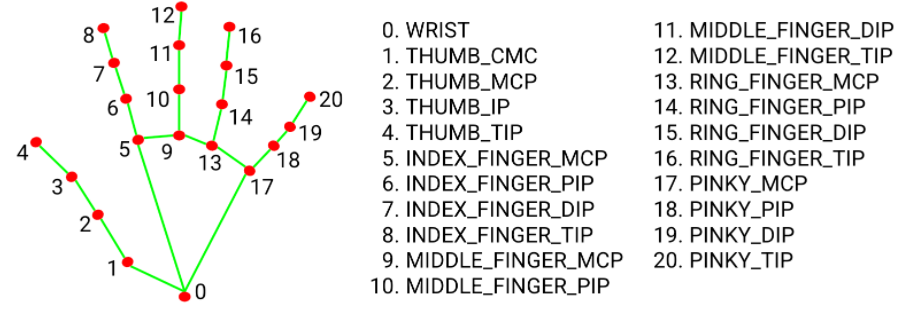
\includegraphics[width=0.9\linewidth]{Nano33BLESense/Hand Landmarks}
	\caption{Hand Landmarks}
	\label{Hand Landmarks}
\end{figure} 

\subsection{Face Detection}
MediaPipe Face Detection is an ultrafast face detection solution that can detect 6 landmarks on the face and also support multiple faces. Fig\ref{Face Detection Using Landmarks} shows the detection of multiple faces using landmarks. The detector’s super-realtime performance enables it to be applied to any live viewfinder experience that requires an accurate facial region of interest as an input for other task-specific models, such as 3D facial keypoint or geometry estimation (e.g., MediaPipe Face Mesh), facial features or expression classification, and face region segmentation. \href{https://google.github.io/mediapipe/solutions/face_detection.html}{Face Detection}

\begin{figure}[h]
	\centering
	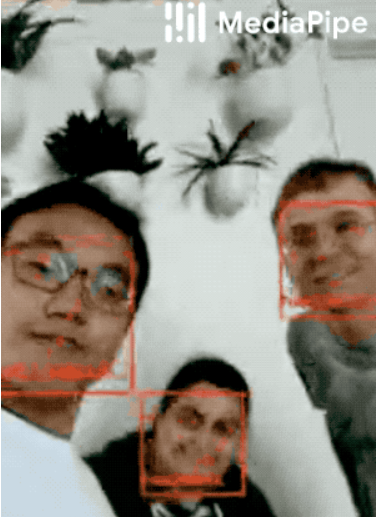
\includegraphics[width=0.5\linewidth]{Nano33BLESense/Face Detection}
	\caption{Face Detection Using Landmarks}
	\label{Face Detection Using Landmarks}
\end{figure}

\subsection{MediaPipe Holistic}

The MediaPipe Holistic pipeline integrates separate models for pose, face and hand components, each of which are optimized for their particular domain.Fig\ref{Face, Pose, and Hand Landmarks} the detection of face, hand, and pose:

\begin{figure}[h]
	\centering
	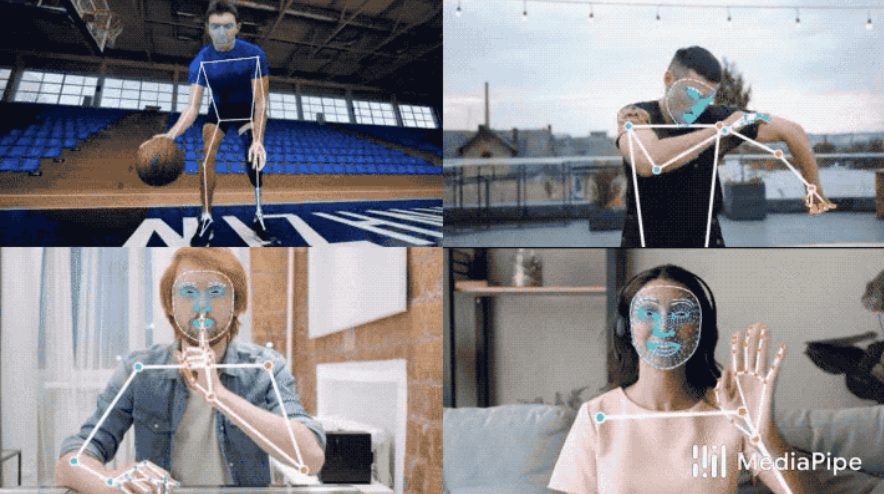
\includegraphics[width=0.7\linewidth]{Nano33BLESense/Holistic}
	\caption{Face, Pose, and Hand Landmarks}
	\label{Face, Pose, and Hand Landmarks}
\end{figure}

MediaPipe holistic offers fast and accurate, yet separate, solutions for these tasks. Combining them all in real-time into a semantically consistent end-to-end solution is a uniquely difficult problem requiring simultaneous inference of multiple, dependent neural networks.\href{https://google.github.io/mediapipe/solutions/holistic.html}{[Holistic]}

\section{Pyfirmata}

The Firmata library implements the Firmata protocol for communicating with software on the host computer. This allows you to write custom firmware without having to create your own protocol and objects for the programming environment that you are using. PyFirmata is basically a prebuilt library package of python program which can be installed in Arduino to allow serial communication between a python script on any computer and with Arduino.
\begin{itemize}
	\item Firamta Serial communication Protocol work as a mediator between two systems as follow.
	\begin{itemize}
		\item Firmata is use as an intermediate protocol that connects an
		embedded system to a host computer.
		\item Using Pyfirmata, the program will run on host computer and get the
		certain output on embedded Devices.
	\end{itemize}
\end{itemize}

Some of the packages we need to implement this project are only supported by python environment, the edge computer we are working with Arduino Nano 33 BLE Sense have Arduino (IDE), it is the c++ integrated development environment. For running the host computer python program, we need to install Firmata library. It helps serial communication protocol and work as a bridge between two environment c++ and python. Fig\ref{Serial Communication protocol using Pyfirmata} shows the two embedded devices, the one raspberry pi support python program and arduino support c++. For running the python programm on host computer, we can see the result on c++ embedded device arduino. 
\begin{figure}[h]
	\centering
	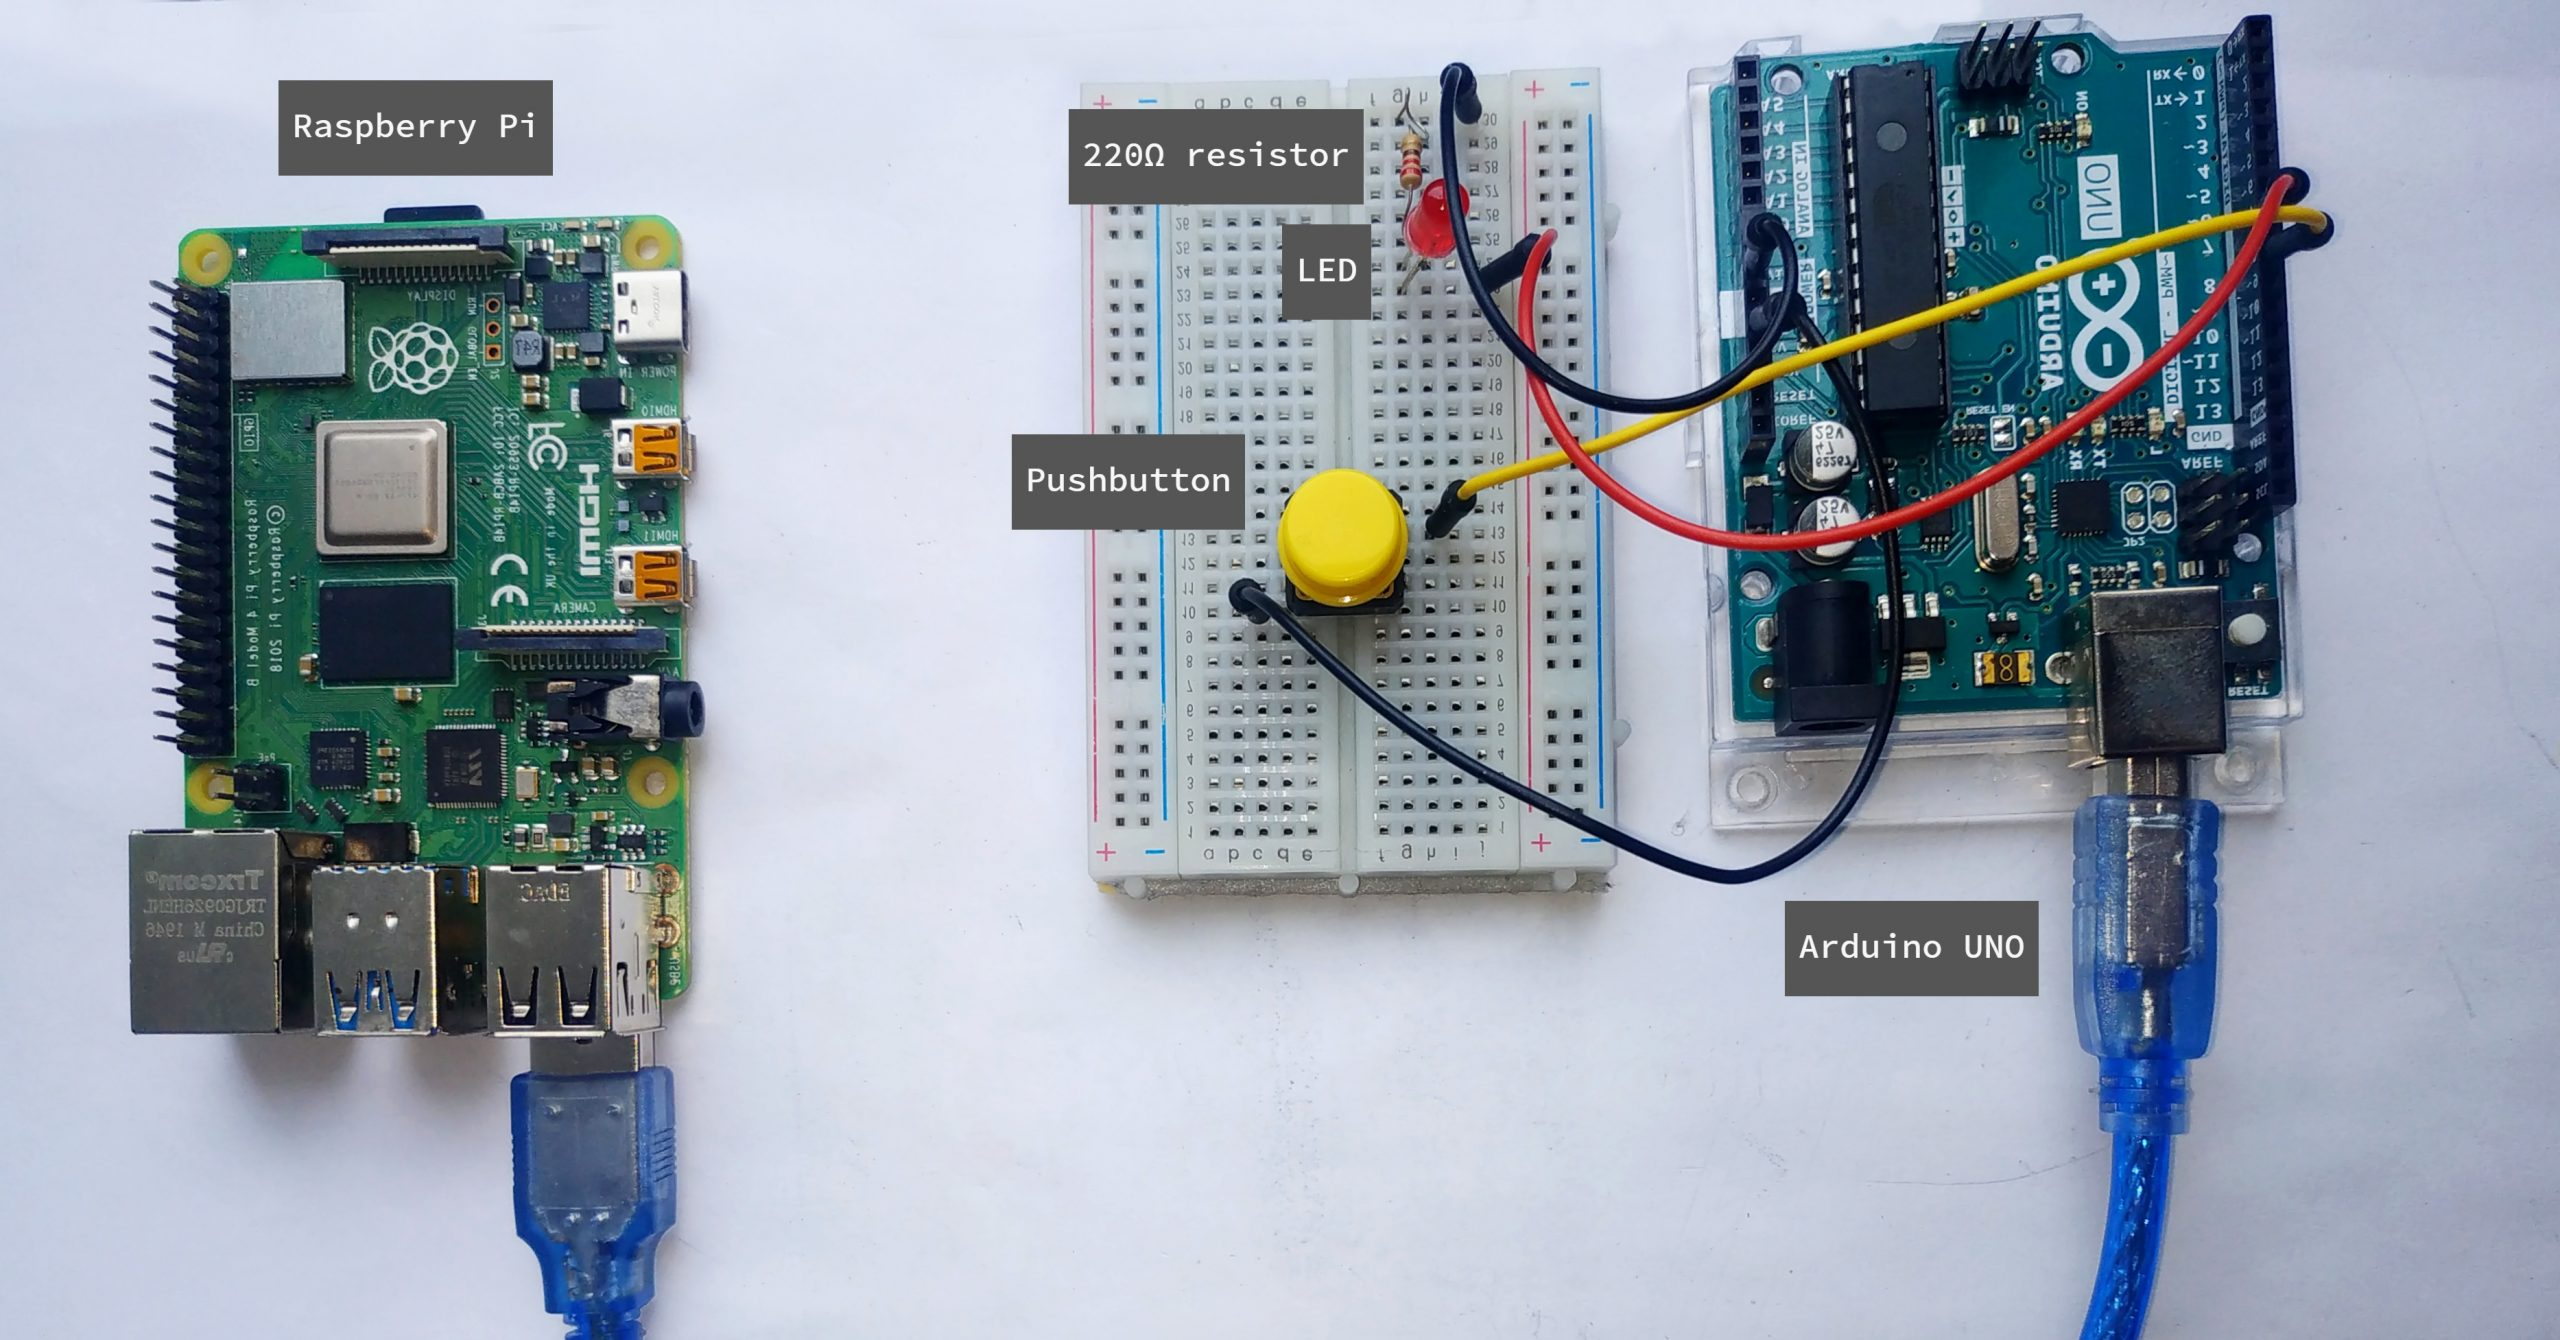
\includegraphics[width=0.7\linewidth]{Nano33BLESense/Pyfirmata}
	\caption{Serial Communication protocol using Pyfirmata}
	\label{Serial Communication protocol using Pyfirmata}
\end{figure}
\section {Supporting Libraries}
Libraries plays a vital role in machine learning and computer vision for training a system. The most important libraries which help us to make mathematical calculation, matrices multiplaction and data visualization and csv files are:
\begin{itemize}
	\item Pandas
	\item Numpy
	\item Matplotlib
	\item Scikit-learn
\end{itemize}
\subsection{Pandas}
Pandas is a Python package providing fast, flexible, and expressive data structures designed to make working with “relational” or “labeled” data both easy and intuitive. It aims to be the fundamental high-level building block for doing practical, real-world data analysis in Python.
\subsection{Numpy}
NumPy is a Python library used for working with arrays. It also has functions for working in domain of linear algebra, fourier transform, and matrices. NumPy was created in 2005 by Travis Oliphant. It is an open source project and you can use it freely. NumPy stands for Numerical Python.
\subsection{Matplotlib}
Matplotlib is a cross-platform, data visualization and graphical plotting library for Python and its numerical extension NumPy. As such, it offers a viable open source alternative to MATLAB. Developers can also use matplotlib's APIs (Application Programming Interfaces) to embed plots in GUI applications.
\subsection{Scikit-learn}
Scikit-learn is arguably the most important library in Python for machine learning. After cleaning and manipulating your data with Pandas or NumPy, scikit-learn is used to build machine learning models as it has tons of tools used for predictive modelling and analysis. There are many reasons to use scikit-learn.
\section{Important Libraries for Arduino Nano 33 BLE Sense}
The Arduino integrated development environment (IDE) comes with a set of standard libraries for commonly used functionality. By installing these libraries it make us in our code more funcnality. These are the following set of libraries which are most commonly suited for our edge computing application.\\
\subsection{Tensor flow lite}
For training the ML Algorithm we will install the Tenson flow lite library on Arduino Nano 33 BLE sense with the help of Integrated Development Environment (IDE) software. It is flexile integrated environment who helps both the software and hardware related to arduino. TensorFlow is an open source library for numerical computation and large-scale machine learning. It make ease in the process of acquiring data, training models, serving predictions, and refining future results.By having this tensor flow lite library, we can deploy or train the ML model. \\
\subsection{ArduCAM}
This is a opensource library for taking high resolution images and short video clip on Arduino based platforms using ArduCAM OV2640 Mini 2MP camera module. For deploying this library on arduino and arducam is available at \url{https://github.com/ArduCAM/Arduino}. We need to select the desire hardware setting about our edge computer and available camera module in the (.h) file.
\subsection{ADPS 9960}
It is the build in Arduino Library for making use of Gesture, Proximity and RGB color detection sensor.



%todo	
%\begin{enumerate}
%	\item ONNX
%	\item Torch
%	\item Accord.NET
%
%	\item Apache Spark
%	\item Apache Mathout
%	\item Apache SINGA
%    \item Apache SystemML \cite{Pansare:2018}
%	
%	\item Gensim
%	\item mlpack
%	\item Mycroft
%	\item DyNet
%	\item Shogun
%\end{enumerate}
